\documentclass[10pt,a4paper]{article}

\usepackage{kotex}
\usepackage[a4paper,margin=17mm]{geometry}
\usepackage{graphicx}
\usepackage{booktabs}
\usepackage{array}
\usepackage{tabularx}
\usepackage{multirow}
\usepackage{subcaption}
\usepackage{caption}
\usepackage{xcolor}
\usepackage{tikz}
\usepackage{pgfplots}
\usepackage{hyperref}
\usepackage{enumitem}
\usepackage{float}
\usepackage{adjustbox}
\usepackage{placeins}

\usetikzlibrary{arrows.meta,positioning,fit}
\pgfplotsset{compat=1.18}
\hypersetup{colorlinks=true,linkcolor=black,citecolor=black,urlcolor=blue}
\captionsetup{font=small,labelfont=bf}
\setlist[itemize]{leftmargin=1.2em,itemsep=0.12em,topsep=0.15em}
\setlength{\parskip}{0.22em}
\setlength{\parindent}{0.8em}
\renewcommand{\arraystretch}{1.10}
\setcounter{topnumber}{5}
\setcounter{bottomnumber}{5}
\setcounter{totalnumber}{8}
\renewcommand{\topfraction}{0.92}
\renewcommand{\bottomfraction}{0.85}
\renewcommand{\textfraction}{0.06}
\renewcommand{\floatpagefraction}{0.80}

\title{\vspace{-1.7em}\textbf{D3Net-based All-in-One Restoration for Smartphone Images with Dirty Lenses}}
\author{20223081 신준철 \\ Deep Learning Programming}
\date{}

\begin{document}
\maketitle
\vspace{-1.4em}

\begin{abstract}
스마트폰 카메라는 일상적으로 사용되지만 렌즈 표면의 dust, fingerprint, scratch, water drop과 같은 오염에 의해 복합적인 영상 열화를 겪는다.
본 프로젝트는 all-in-one image restoration 모델인 D3Net을 SIDL dirty lens restoration에 적용하고, patch size와 refinement strategy가 복원 성능에 미치는 영향을 분석한다.
256$\times$256 crop으로 continued training한 epoch 73 D3Net checkpoint를 SIDL official leaderboard test set에 제출한 결과, 24.55 dB / SSIM 0.8507을 달성하였다.
128$\times$128 baseline은 23.33 dB / 0.8357로 낮았고, 256 best checkpoint에서 시작한 512$\times$512 refinement는 23.27 dB / 0.8336으로 하락하였다.
결과는 dirty lens artifact 복원에 충분한 spatial context가 중요하지만, 큰 patch가 항상 유리하지는 않으며 crop distribution, augmentation, batch dynamics, optimization stability 사이의 trade-off가 존재함을 보여준다.
\end{abstract}

\section{Introduction}
Dirty lens restoration은 일반적인 denoising 또는 deblurring과 다르다.
스마트폰 렌즈 표면의 오염은 장면 자체의 blur나 sensor noise가 아니라 렌즈 앞의 물리적 contamination에서 발생하므로, spatial artifact와 frequency-domain artifact가 동시에 나타난다.
예를 들어 dust는 국소적인 산란과 contrast 저하를 만들고, fingerprint나 mixed contamination은 저주파 haze와 고주파 edge 손실을 함께 유발할 수 있다.
SIDL은 이러한 문제를 실제 스마트폰 촬영 환경에서 paired clean/degraded image로 구성한 dirty lens restoration dataset이다 \cite{choi2025sidl}.

본 프로젝트의 핵심 질문은 다음과 같다.
\textit{All-in-one image restoration model인 D3Net이 SIDL dirty lens restoration에 효과적으로 적용될 수 있는가?}
또한 \textit{patch size와 refinement strategy는 성능에 어떤 영향을 주며, Hard difficulty 특히 Dust/Mixed contamination에서 병목이 왜 발생하는가?}를 분석한다.

본 보고서의 기여는 세 가지다.
첫째, D3Net \cite{wang2025d3net}을 SIDL dirty lens restoration에 적용하여 제한된 프로젝트 예산에서 scratch adaptation을 수행하였다.
둘째, 128/256/512 patch-size 및 refinement strategy를 비교하여 256$\times$256 crop training이 가장 안정적임을 확인하였다.
셋째, difficulty/type별 validation breakdown을 통해 최종 성능 병목이 Hard Dust와 Hard Mixed 계열에 집중됨을 보였다.

본 보고서는 SIDL 데이터셋에서 SOTA 성능을 달성하는 것을 목표로 하지 않았다. 대신 D3Net이라는 degradation-adaptive all-in-one backbone을 SIDL에 적용했을 때 어떤 조건에서 안정적으로 학습되는지, 그리고 어떤 조건에서 성능이 무너지는지를 분석하는 adaptation study로 해석한다.

\section{Related Work and Background}
\textbf{SIDL dataset.}
SIDL은 Smartphone Images with Dirty Lenses의 약자로, 스마트폰 렌즈 오염 복원을 위한 real-world paired dataset이다 \cite{choi2025sidl}.
오염 유형은 clean, dust, fingerprint/finger, mixed, scratch, water를 포함하며, 평가 난이도는 Easy, Medium, Hard로 나뉜다.
본 프로젝트에서는 512$\times$512로 patchified된 SIDL image pair를 사용하였다.
학습에는 train split의 degraded-clean pair를 사용하고, validation은 type과 difficulty가 분리된 512$\times$512 image pair에서 PSNR/SSIM으로 수행하였다.

\textbf{All-in-one dirty lens baselines.}
SIDL 논문은 AirNet, NAFNet, Restormer, FFTformer, DiffUIR, MambaIR 등을 포함해 dirty lens restoration에서 여러 복원 모델을 비교한다.
이 중 본 보고서에서 특히 비교 맥락으로 보는 모델은 AirNet과 DiffUIR이다.
AirNet은 all-in-one restoration 관점에서 비교된 CNN 계열 baseline이고, DiffUIR는 diffusion 기반 universal restoration 모델로 SIDL에서 강한 결과를 보인 방법이다.
따라서 본 프로젝트의 D3Net 결과를 해석할 때, 단순한 PSNR 수치 경쟁보다도 ``all-in-one 방식이 dirty lens contamination을 얼마나 일반화할 수 있는가''라는 관점이 중요하다.

\textbf{D3Net.}
D3Net은 Dynamic Degradation Decomposition Network의 약자로, frequency-domain degradation cue와 prompt-guided dynamic decomposition을 통해 여러 degradation type을 하나의 모델로 복원하려는 all-in-one restoration architecture이다 \cite{wang2025d3net}.
D3Net 원 논문은 128$\times$128 crop으로 장기간 학습한 설정을 사용하며, 저자가 확인한 official training setting은 약 1200 epochs 수준이다.
반면 본 프로젝트의 main run은 256$\times$256 crop으로 수행되었고 64 epoch에서 early stopping되었으므로, 원 논문 수준의 충분한 장기 학습과 직접 비교할 수 없다.
이 한계는 결과 해석에서 중요하다. 즉 현재 성능은 D3Net 구조 자체의 상한이라기보다, 제한된 compute budget에서 SIDL에 scratch adaptation한 결과에 가깝다.

\section{Method}
그림 \ref{fig:d3net}은 본 프로젝트에서 사용한 D3Net pipeline을 요약한다.
모델은 U-Net style encoder-decoder 구조를 기반으로 하며, 입력 dirty image에서 직접 clean image를 예측하기보다 residual correction을 예측한다.
최종 출력은 입력 영상 $x$와 모델이 예측한 residual $r_\theta(x)$의 합으로 계산된다.
\begin{equation}
    \hat{y} = x + r_\theta(x).
\end{equation}
이 residual formulation은 dirty input의 장면 구조를 보존하면서 contamination으로 인한 local/global artifact를 보정하는 방향으로 학습을 유도한다.

\begin{figure}[H]
    \centering
    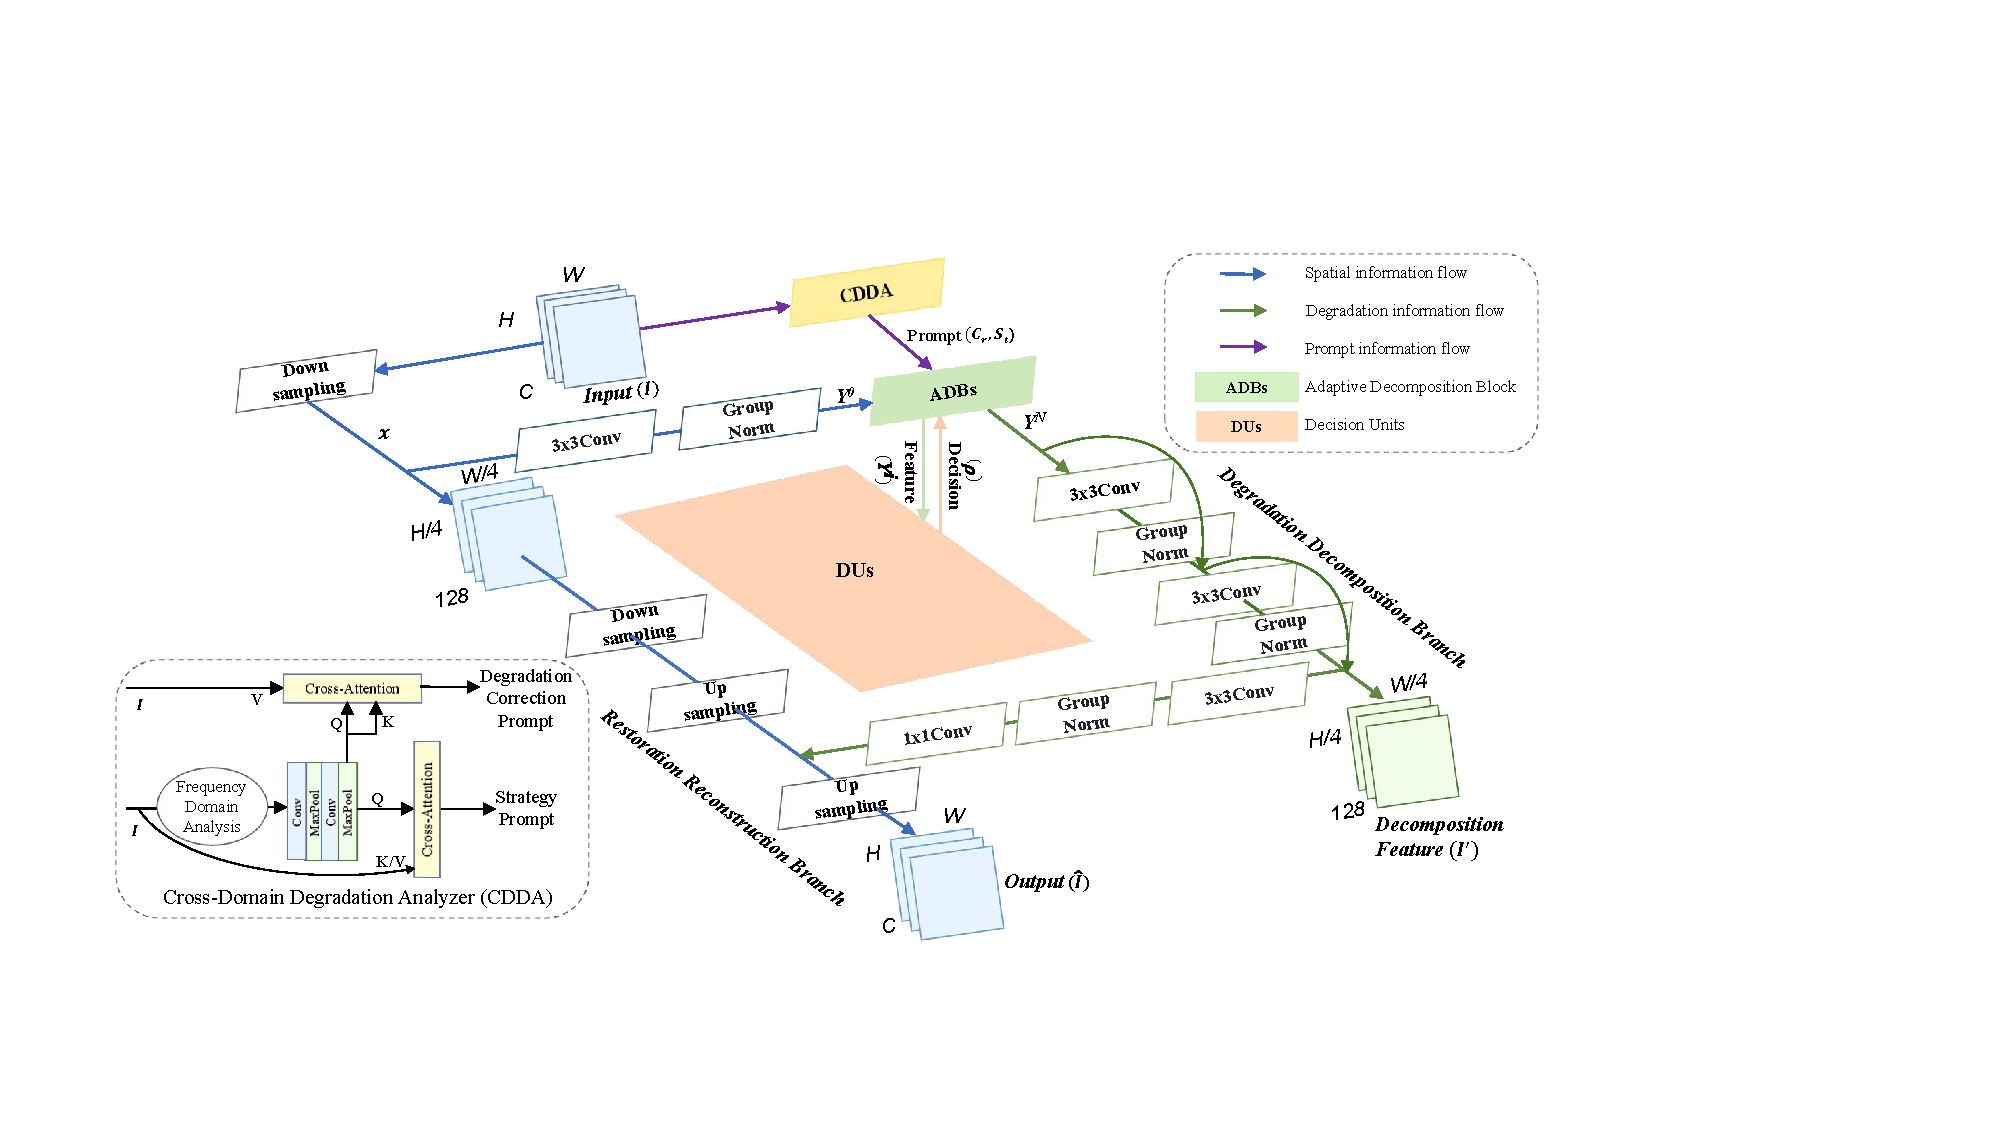
\includegraphics[width=0.92\linewidth,height=0.30\textheight,keepaspectratio]{figures/d3net_architecture_paper.pdf}
    \caption{D3Net architecture from the original paper \cite{wang2025d3net}. 모델은 restoration reconstruction branch와 degradation decomposition branch로 구성되며, CDDA가 degradation correction prompt와 strategy prompt를 생성한다.}
    \label{fig:d3net}
\end{figure}

\textbf{Encoder--decoder reconstruction branch.}
D3Net의 reconstruction branch는 multi-scale feature extraction과 skip connection을 사용하는 encoder--decoder 계열 구조이다.
Encoder는 입력 영상을 단계적으로 downsampling하면서 local texture, edge, low-frequency illumination pattern을 feature로 추출한다.
Decoder는 이러한 feature를 다시 고해상도 복원 결과로 변환하고, skip connection은 dirty lens 오염이 상대적으로 약한 영역의 장면 구조와 경계 정보를 보존하는 데 도움을 준다.
Dirty lens restoration에서는 원본 장면 자체는 보존되어야 하고 오염으로 인한 residual만 제거되어야 하므로, residual learning과 encoder--decoder 구조의 조합이 자연스럽다.

\textbf{Fourier degradation cue.}
D3Net의 중요한 특징은 입력 영상을 spatial domain만으로 보지 않고 frequency domain cue를 함께 사용한다는 점이다.
Fourier branch는 입력 이미지의 FFT magnitude 또는 frequency representation을 기반으로 degradation feature를 추출한다.
Dust나 scratch는 국소적 고주파 artifact와 edge distortion을 만들 수 있고, fingerprint, water, mixed contamination은 저주파 haze, contrast shift, local blur를 동시에 만들 수 있다.
따라서 frequency cue는 단순한 RGB texture만으로는 구분하기 어려운 contamination pattern을 모델에 제공하는 역할을 한다.

\textbf{CDDA prompt and cross-attention.}
D3Net은 frequency feature와 image feature 사이의 상호작용을 통해 degradation-aware prompt를 만든다.
원 논문 구조에서 CDDA는 correction prompt와 strategy prompt를 생성하며, 이 prompt는 reconstruction branch의 feature processing에 조건으로 사용된다.
Cross-attention module은 degradation cue가 image feature의 어느 위치와 채널에 중요하게 작용해야 하는지를 학습한다.
SIDL에서는 하나의 이미지 안에서도 water drop, fingerprint residue, dust particle이 서로 다른 위치와 scale로 나타날 수 있으므로, global degradation label보다 feature-level prompt가 더 유연하다.

\textbf{Dynamic Degradation Decomposition Block.}
DDB는 D3Net의 핵심적인 adaptive processing module이다.
DDB 내부의 Decision Unit(DU)은 prompt와 image feature를 이용해 Adaptive Decomposition Block(ADB)을 적용할지 결정한다.
즉 모든 sample과 모든 feature가 같은 연산 경로를 거치는 것이 아니라, degradation cue에 따라 필요한 feature transformation을 선택적으로 적용한다.
ADB는 prompt-conditioned operation을 통해 오염 제거에 필요한 feature 변환을 수행한다.
이러한 동적 구조는 SIDL처럼 degradation type이 하나로 고정되지 않고 dust, scratch, water, fingerprint, mixed contamination이 섞인 all-in-one restoration 문제에 적용할 의미가 있다.

\begin{figure}[H]
    \centering
    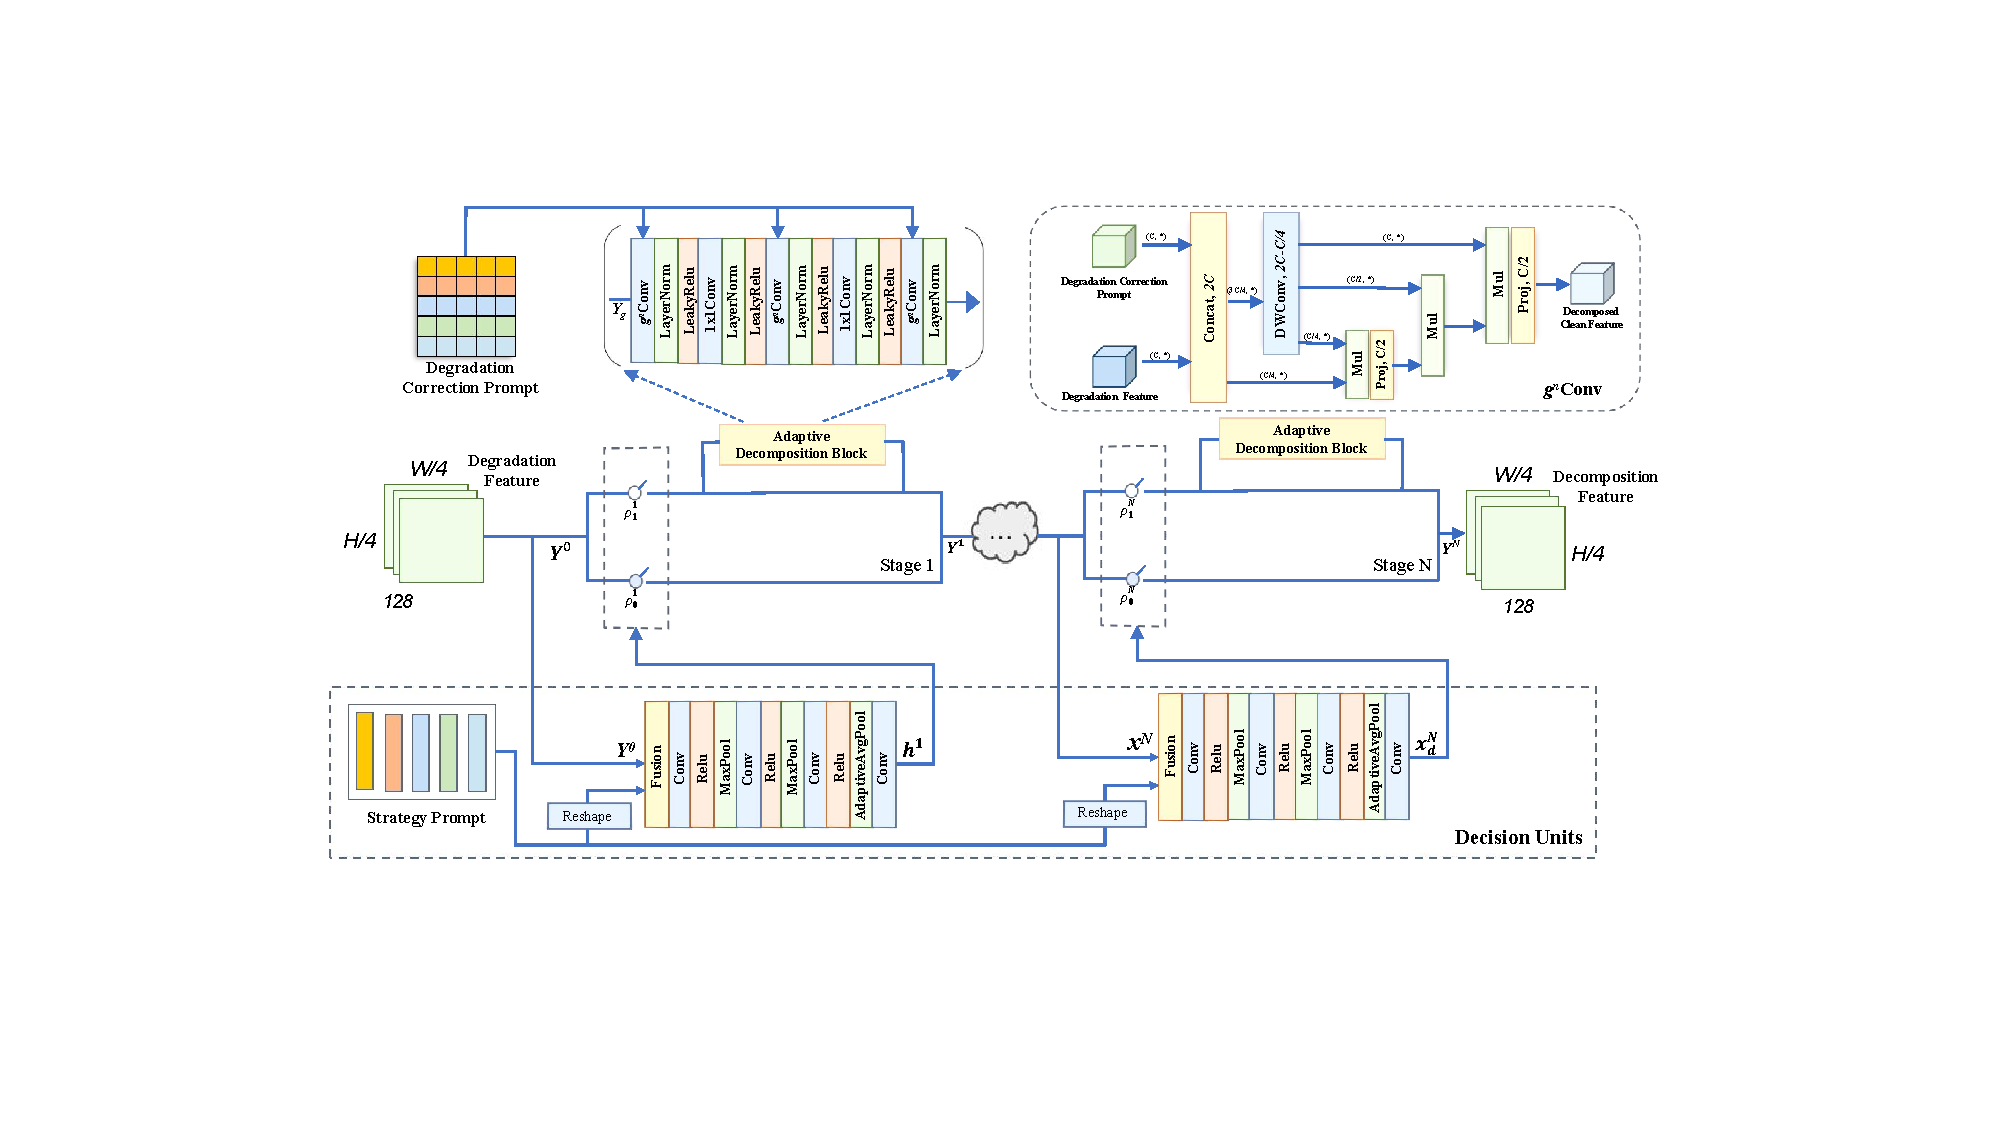
\includegraphics[width=0.70\linewidth,height=0.22\textheight,keepaspectratio]{figures/d3net_ddm_paper.pdf}
    \caption{Dynamic Decomposition Mechanism from the original D3Net paper \cite{wang2025d3net}. DUs는 ADB 활성 여부를 결정하고, ADBs는 prompt-conditioned feature transformation을 수행한다.}
    \label{fig:ddm}
\end{figure}

\section{Experimental Setup}
\textbf{Dataset.}
실험에는 SIDL의 512$\times$512 patchified degraded-clean pair를 사용하였다.
Train split은 contamination type별 input/target pair로 구성되며, validation split은 type과 difficulty(Easy/Medium/Hard) 기준으로 분리되어 있다.
Validation은 full 512$\times$512 center crop 기준으로 수행하였다.

\textbf{Training configuration.}
메인 실험은 D3Net을 pretrained checkpoint 없이 scratch training한 결과이다.
256$\times$256 crop run은 fixed final dataset에서 수행한 main controlled experiment이고, 기존 best validation checkpoint는 epoch 34에서 23.82 dB / 0.8398을 기록하였다.
이후 latest checkpoint에서 256$\times$256 continued training을 수행한 결과 epoch 73 checkpoint를 official leaderboard에 제출하였고, test-set 기준 24.55 dB / 0.8507을 얻었다.
Loss는 normalized RGB tensor 기준 L1 loss를 사용하였고, optimizer는 Adam($\beta_1=0.9,\beta_2=0.999$) 및 cosine annealing scheduler를 사용하였다.
학습 하드웨어는 single RTX 4090이다.
Validation에서는 D3Net이 예측한 residual을 입력 영상에 더해 최종 복원 영상을 생성하였다.
이후 restored output과 target을 ImageNet mean/std 기준으로 denormalize하고 $[0,1]$ 범위로 clamp한 뒤 PSNR/SSIM을 image-wise로 계산하였다.
각 image 단위 metric은 contamination type과 difficulty level 기준으로 평균 집계하였다.
본 실험은 official D3Net 수준으로 충분한 epoch를 사용해 완전 수렴시킨 연구가 아니라, 수업 프로젝트의 제한된 시간과 compute budget 안에서 수행한 adaptation이다.

PSNR은 복원 영상과 GT 영상 사이의 mean squared error를 기반으로 pixel-level fidelity를 측정한다.
본 실험에서는 denormalized image를 $[0,1]$ 범위로 clamp한 뒤 PSNR을
\begin{equation}
    \mathrm{PSNR} = 20 \log_{10}\left(\frac{1}{\sqrt{\mathrm{MSE}}}\right)
\end{equation}
로 계산하였다.
SSIM은 luminance, contrast, structure를 고려하여 복원 영상이 GT 구조를 얼마나 보존하는지 평가하는 지표이다.

\textbf{Ablation design.}
128$\times$128 crop baseline은 초기 실험으로, incremental task/data addition이 있었기 때문에 완전히 통제된 비교는 아니다.
그러나 작은 patch의 context 부족을 보여주는 exploratory baseline으로 포함한다.
256$\times$256 run은 최종 고정 dataset에서 수행한 main controlled experiment이다.
512$\times$512 refinement는 256 best checkpoint에서 시작하였고, learning rate는 $1\times10^{-5}$, training batch size는 1로 설정되었다.
256 low-LR polishing 역시 256 best checkpoint에서 시작한 추가 fine-tuning 실험이다.

\section{Results}
\begin{table}[H]
\centering
\caption{Reference comparison with existing all-in-one restoration models reported in the original D3Net paper \cite{wang2025d3net}. The benchmark averages five restoration tasks (Rain100L, SOTS, BSD68, GoPro, LOL), so it is not directly comparable to our SIDL validation numbers.}
\label{tab:allinone_context}
\small
\begin{tabularx}{\linewidth}{l c c c X}
\toprule
Method & Avg. PSNR & Avg. SSIM & Params / FLOPs & Interpretation \\
\midrule
AirNet & 25.49 & 0.846 & 8.93M / 75.32G & Contrastive/degradation-aware all-in-one baseline. \\
PromptIR & 27.57 & 0.881 & 32.97M / 370.64G & Prompt-based restoration with high computational cost. \\
IDR & 28.34 & 0.893 & 15.34M / -- & Ingredient-oriented multi-degradation formulation. \\
InstructIR & 29.55 & 0.907 & 15.84M / 37.95G & Text-instructed restoration; depends on predefined instructions. \\
D3Net & \textbf{32.36} & 0.901 & 37.80M / 33.67G & Frequency-domain CDDA + dynamic decomposition; selected as the SIDL adaptation backbone. \\
\bottomrule
\end{tabularx}
\end{table}


표 \ref{tab:allinone_context}는 본 프로젝트에서 새로 측정한 SIDL 결과가 아니라 D3Net 원 논문의 five-task all-in-one benchmark를 요약한 reference comparison이다.
따라서 본 프로젝트의 SIDL validation 결과와 직접적인 순위 비교로 해석하면 안 된다.
이 표는 D3Net을 선택한 근거, 즉 frequency-domain cue와 dynamic decomposition을 사용하는 degradation-adaptive backbone이라는 점을 설명하기 위한 제한적 참고 자료이다.

\begin{table}[H]
\centering
\caption{SIDL paper-style baseline comparison. AirNet and DiffUIR values are from the SIDL paper test-set table, while D3Net values are from our epoch-73 validation checkpoint using continued 256 crop training. Because the split and training budget differ, this table is used as task context rather than a strict leaderboard comparison.}
\label{tab:sidl_airnet_diffuir}
\tiny
\setlength{\tabcolsep}{2.4pt}
\renewcommand{\arraystretch}{0.96}
\resizebox{\linewidth}{!}{%
\begin{tabular}{lllcccccc|c}
\toprule
\textbf{Method} & \textbf{Network} & &
\textbf{Clean} &
\textbf{Dust} &
\textbf{Fingerprint} &
\textbf{Water} &
\textbf{Scratch} &
\textbf{Mixed} &
\textbf{Average} \\
& & &
PSNR/SSIM &
PSNR/SSIM &
PSNR/SSIM &
PSNR/SSIM &
PSNR/SSIM &
PSNR/SSIM &
PSNR/SSIM \\
\midrule
\multirow{3}{*}{CNN}
& \multirow{3}{*}{AirNet\textsuperscript{\dag}}
& Easy   & 27.10 / 0.9329 & 23.40 / 0.8669 & 25.10 / 0.8708 & 24.85 / 0.8658 & 25.84 / 0.8917 & 25.30 / 0.8422 & 25.26 / 0.8784 \\
& & Medium & 26.13 / 0.8899 & 19.69 / 0.7577 & 22.53 / 0.8191 & 20.36 / 0.7656 & 21.24 / 0.8051 & 16.79 / 0.7542 & 21.12 / 0.7986 \\
& & Hard   & 23.79 / 0.8527 & 16.18 / 0.7350 & 15.83 / 0.6432 & 16.64 / 0.7449 & 18.13 / 0.7975 & 14.48 / 0.7047 & 17.50 / 0.7463 \\
\midrule
\multirow{3}{*}{Diffusion}
& \multirow{3}{*}{DiffUIR\textsuperscript{\dag}}
& Easy   & 34.51 / 0.9785 & 26.96 / 0.9276 & 28.82 / 0.9331 & 27.42 / 0.9220 & 30.14 / 0.9375 & 28.22 / 0.9021 & 29.34 / 0.9335 \\
& & Medium & 33.25 / 0.9375 & 22.11 / 0.8325 & 26.16 / 0.8856 & 24.65 / 0.8647 & 27.07 / 0.9105 & 20.32 / 0.8368 & 25.36 / 0.8786 \\
& & Hard   & 29.47 / 0.9366 & 20.38 / 0.8602 & 18.93 / 0.7763 & 19.91 / 0.8500 & 21.27 / 0.8599 & 18.97 / 0.8409 & 21.71 / 0.8533 \\
\midrule
\multirow{3}{*}{Ours}
& \multirow{3}{*}{D3Net}
& Easy   & 32.78 / 0.9542 & 25.07 / 0.8859 & 24.59 / 0.7733 & 26.38 / 0.9196 & 27.84 / 0.8980 & 23.32 / 0.8552 & 26.66 / 0.8810 \\
& & Medium & 30.26 / 0.9424 & 24.03 / 0.8797 & 23.69 / 0.8467 & 24.05 / 0.8577 & 27.41 / 0.9126 & 22.56 / 0.8869 & 25.33 / 0.8877 \\
& & Hard   & 27.70 / 0.8502 & 17.05 / 0.7086 & 20.23 / 0.7698 & 20.22 / 0.7986 & 20.38 / 0.7477 & 17.98 / 0.7900 & 20.59 / 0.7775 \\
\bottomrule
\end{tabular}}
\end{table}


표 \ref{tab:sidl_airnet_diffuir}는 SIDL 논문에서 제시한 AirNet과 DiffUIR baseline을 논문 Table 2 형식에 맞춰 정리하고, 본 프로젝트의 epoch 73 D3Net 256 crop 결과를 같은 contamination type 및 difficulty 축에 함께 배치한 것이다.
AirNet과 DiffUIR는 SIDL 논문의 test-set 결과이고, D3Net은 본 프로젝트의 official leaderboard submission 결과이다.
따라서 이 표는 기존 baseline의 성능 범위 안에서 D3Net adaptation 결과가 어떤 difficulty/type에서 강하거나 약한지 해석하기 위한 context로 사용한다.

\begin{table}[H]
\centering
\caption{Validation summary of D3Net SIDL experiments. 확인되지 않은 추가 결과는 포함하지 않았다.}
\label{tab:main}
\small
\begin{tabularx}{\linewidth}{l c c c c X}
\toprule
Run & Train crop & Best epoch & PSNR & SSIM & Notes \\
\midrule
128 crop baseline & 128 & 34 & 23.33 & 0.8357 & 초기 exploratory baseline; incremental task/data addition으로 완전 통제 실험은 아님 \\
256 crop main & 256 & 34 & \textbf{23.82} & 0.8398 & fixed final dataset에서 수행한 main controlled run \\
256 low-LR polishing & 256 & 3 & 23.76 & \textbf{0.8409} & 256 best에서 LR $1\times10^{-5}$로 fine-tuning; PSNR은 main run 미달 \\
512 refinement & 512 & 2 & 23.27 & 0.8336 & 256 best에서 LR $1\times10^{-5}$, batch size 1로 refinement; negative result \\
\bottomrule
\end{tabularx}
\end{table}

\begin{table}[H]
\centering
\caption{256 crop main run의 difficulty-wise validation breakdown.}
\label{tab:difficulty}
\small
\begin{tabular}{lcc}
\toprule
Difficulty & PSNR (dB) & SSIM \\
\midrule
Easy & 27.00 & 0.8812 \\
Medium & 25.36 & 0.8862 \\
Hard & 20.33 & 0.7743 \\
\midrule
Overall & \textbf{23.82} & \textbf{0.8398} \\
\bottomrule
\end{tabular}
\end{table}

\begin{table}[H]
\centering
\caption{256 crop main run의 contamination type-wise validation average.}
\label{tab:type}
\small
\begin{tabular}{lcc}
\toprule
Type & PSNR (dB) & SSIM \\
\midrule
Clean & 29.93 & 0.9113 \\
Dust & 21.89 & 0.8203 \\
Finger & 21.80 & 0.7858 \\
Mixed & 20.48 & 0.8269 \\
Scratch & 25.07 & 0.8488 \\
Water & 22.93 & 0.8423 \\
\bottomrule
\end{tabular}
\end{table}


256$\times$256 continued training의 epoch 73 checkpoint는 official leaderboard test set에서 24.55 dB / 0.8507을 기록하였다.
해당 제출의 model complexity는 771 GMACs, parameter 수는 43.8M으로 보고되었다.
128 baseline은 23.33 dB / 0.8357에 그쳤고, 512 refinement는 23.27 dB / 0.8336으로 하락하였다.
256 low-LR polishing은 SSIM은 0.8409까지 상승했으나 PSNR은 23.76 dB로 epoch 73 continued checkpoint를 넘지 못했다.
이 결과는 단순히 입력 crop을 크게 만드는 것이 성능 향상으로 이어지지 않음을 보여준다.
128 crop은 학습 안정성 측면에서는 부담이 작지만, dirty lens degradation처럼 넓은 영역의 contrast 변화와 local artifact가 함께 나타나는 문제에서는 충분한 주변 문맥을 제공하지 못할 수 있다.
반대로 512 crop refinement는 전체 patch를 더 넓게 볼 수 있다는 장점이 있지만, batch size가 1로 줄어드는 조건에서는 gradient가 불안정해지고 random crop augmentation 효과도 약해진다.
따라서 본 실험에서 256 crop은 spatial context, augmentation diversity, batch stability 사이의 가장 현실적인 균형점으로 해석된다.

Low-LR polishing 결과도 비슷한 결론을 뒷받침한다.
Epoch-34 256 best checkpoint에서 learning rate를 $1\times10^{-5}$로 낮춰 추가 학습했을 때 SSIM은 0.8398에서 0.8409로 소폭 상승했지만, PSNR은 23.82 dB에서 23.76 dB로 감소하였다.
이는 추가 학습이 구조적 유사도에는 약간 유리하게 작용했을 수 있으나, pixel-level fidelity 관점에서는 이미 main checkpoint가 더 좋은 균형에 도달했음을 의미한다.
반면 latest checkpoint에서 이어간 256 continued training은 official test set에서 가장 높은 최종 제출 성능을 보였으므로, 현재 보고서의 최종 후보는 epoch 73 checkpoint로 갱신한다.

Official leaderboard 기준 difficulty average는 Easy 28.02 dB / 0.9051, Medium 24.70 dB / 0.8407, Hard 20.92 dB / 0.8064이다.
Hard split은 여전히 가장 낮은 성능 영역이며, 이는 all-in-one restoration에서 심한 오염과 약한 오염을 동시에 다루는 것이 어렵다는 점을 보여준다.

\begin{figure}[H]
    \centering
    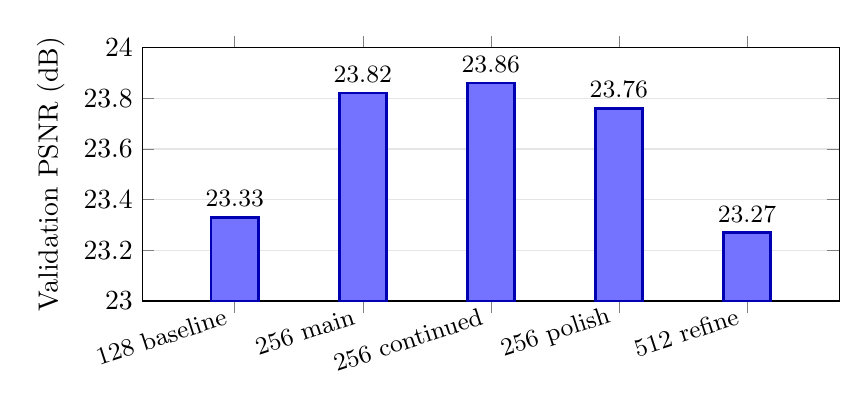
\begin{tikzpicture}
\begin{axis}[
    width=0.86\linewidth,
    height=4.8cm,
    ymin=23.0,
    ymax=24.0,
    ymajorgrids=true,
    grid style={black!10},
    symbolic x coords={128 baseline,256 main,256 continued,256 polish,512 refine},
    xtick=data,
    x tick label style={rotate=18,anchor=east,font=\small},
    ylabel={Validation PSNR (dB)},
    nodes near coords,
    nodes near coords style={font=\small},
    every axis plot/.append style={line width=0.9pt},
    bar width=17pt,
    ybar,
    enlarge x limits=0.18,
]
\addplot[fill=blue!55,draw=blue!70!black] coordinates {
    (128 baseline,23.33)
    (256 main,23.82)
    (256 continued,23.86)
    (256 polish,23.76)
    (512 refine,23.27)
};
\end{axis}
\end{tikzpicture}

    \caption{Patch-size/refinement ablation. 256 continued training이 가장 높은 validation PSNR을 달성하였고, 512 refinement는 더 큰 context에도 불구하고 성능이 하락하였다.}
    \label{fig:ablation}
\end{figure}

Difficulty-wise 결과는 Hard split에서 큰 하락을 보인다.
Official leaderboard 기준 Easy average는 28.02 dB / 0.9051, Medium average는 24.70 dB / 0.8407, Hard average는 20.92 dB / 0.8064이다.
Type-wise average에서는 clean이 30.47 dB / 0.9256으로 가장 높고, mixed가 22.19 dB / 0.8261, dust가 22.61 dB / 0.8312, water가 23.22 dB / 0.8357로 낮다.
특히 Hard Fingerprint는 18.09 dB / 0.6940, Hard Mixed는 18.82 dB / 0.8089, Hard Water는 19.47 dB / 0.7950으로 주요 병목에 해당한다.

\begin{figure}[H]
    \centering
    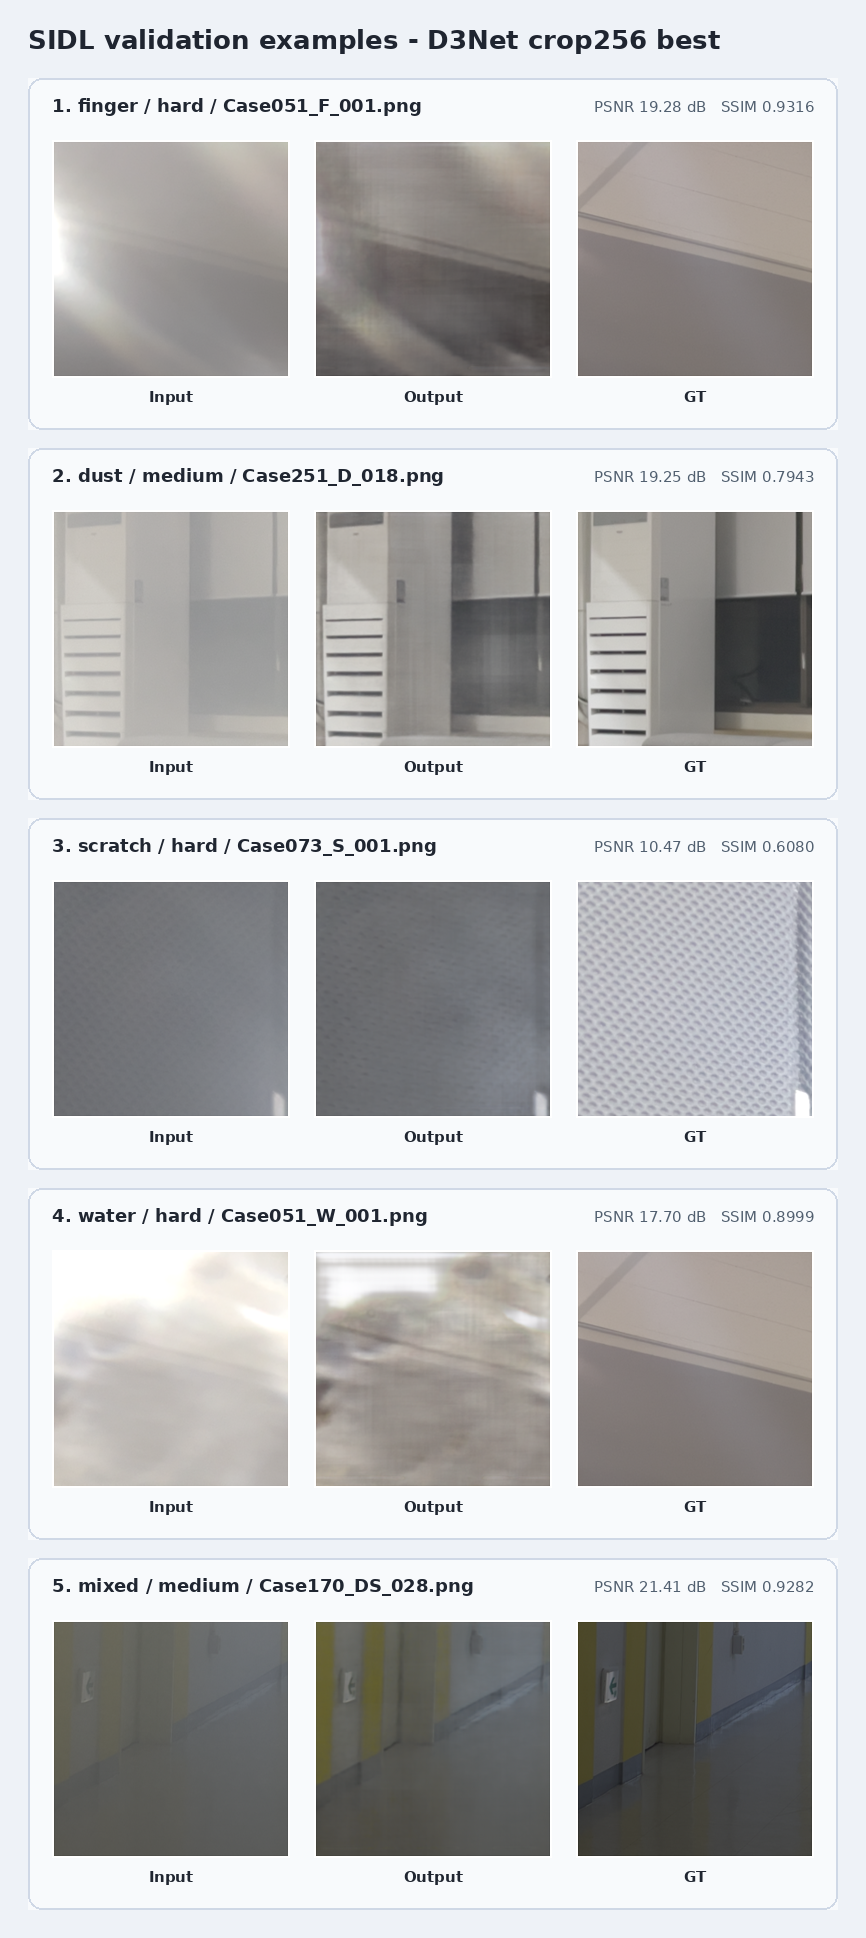
\includegraphics[width=\linewidth,height=0.62\textheight,keepaspectratio]{figures/qualitative_grid_placeholder.png}
    \caption{D3Net qualitative examples. 각 예시는 input / D3Net output / GT 비교 패널이며, finger-hard, dust-medium, scratch-hard, water-hard, mixed-medium sample을 포함한다. The figure is height-limited to prevent page overflow and clipping.}
    \label{fig:qualitative}
\end{figure}
\FloatBarrier

\section{Discussion}
\textbf{Why 256 crop worked best.}
128$\times$128 crop은 dirty lens artifact를 복원하기에 충분한 spatial context를 제공하지 못했을 가능성이 높다.
렌즈 오염은 local texture만의 문제가 아니라 영상 전체의 contrast, veiling, scattering, low-frequency distortion과 연결된다.
특히 water drop이나 fingerprint는 crop 내부의 texture뿐 아니라 주변 배경과의 contrast 관계를 이용해야 복원 방향을 안정적으로 정할 수 있다.
256$\times$256 crop은 local artifact와 주변 context를 함께 볼 수 있으면서도 batch size와 augmentation 다양성을 유지할 수 있어 가장 안정적인 trade-off를 만들었다.
또한 256 crop은 512 patch에서 다양한 위치를 반복적으로 샘플링하기 때문에, 같은 원본 patch에서도 서로 다른 local composition을 학습에 제공한다.
이는 SIDL처럼 오염이 이미지 전체에 균일하게 퍼져 있지 않고 국소적으로 나타나는 경우 중요하다.
예를 들어 dust와 scratch는 특정 위치에 작은 고주파 artifact를 만들고, water나 fingerprint는 넓은 영역의 blur나 contrast shift를 만든다.
256 crop은 이러한 local artifact와 주변 배경을 동시에 포함할 가능성이 높으면서도, 512 full patch보다 더 많은 crop variation을 제공한다.

\textbf{Why 512 refinement failed.}
512$\times$512 refinement는 더 큰 context를 제공하지만 성능은 23.27 dB로 하락했다.
첫 번째 가능성은 effective training distribution shift이다.
256 training은 512 patch에서 random 256 crop을 반복적으로 뽑으므로 augmentation 다양성이 크지만, 512 training은 full patch 학습에 가까워져 모델이 보게 되는 crop distribution이 달라진다.
두 번째는 batch dynamics이다.
512 refinement는 batch size가 1로 줄어 gradient estimate가 불안정해지고, cosine schedule 및 low learning rate 조건에서도 optimization이 민감해질 수 있다.
세 번째는 D3Net의 Fourier/prompt branch가 input scale 또는 crop distribution 변화에 민감할 가능성이다.
따라서 patch size는 단순히 클수록 좋은 hyperparameter가 아니라 spatial context, augmentation, batch size, optimization stability 사이의 균형으로 보아야 한다.
특히 Fourier branch는 입력의 frequency distribution을 활용하므로, crop 크기와 sampling 방식이 바뀌면 모델이 보는 frequency statistics도 달라질 수 있다.
256 crop에서 학습된 checkpoint를 512 crop으로 바로 refine할 경우, reconstruction branch뿐 아니라 degradation prompt를 만드는 branch도 새로운 입력 통계에 적응해야 한다.
이 과정이 충분히 길거나 안정적으로 진행되지 않으면, 더 큰 context가 있어도 실제 validation metric은 낮아질 수 있다.
본 실험의 512 refinement는 epoch 2에서 best를 기록했고 더 긴 안정화 과정을 거치지 못했으므로, 512 crop 자체의 가능성을 완전히 배제하기보다는 현재 compute budget에서 불안정했던 설정으로 해석하는 것이 적절하다.

\textbf{Why sufficient training budget matters.}
D3Net 원 논문은 128$\times$128 crop과 약 1200 epoch 수준의 장기 학습을 사용한 것으로 확인하였다.
이에 비해 본 프로젝트의 main run은 epoch 34에서 기존 best를 기록했고, 이후 continued training을 통해 epoch 73에서 current best를 기록하였다.
그러나 epoch 73 역시 원 D3Net의 장기 학습 규모와 비교하면 매우 짧은 학습이다.
따라서 본 결과는 D3Net의 충분한 수렴 성능이라기보다, 제한된 시간 내 scratch training에서 얻은 성능이다.
D3Net은 dynamic decision과 prompt-conditioned feature transformation을 포함하기 때문에, 짧은 학습에서는 degradation별 routing과 feature decomposition이 충분히 안정화되지 않았을 수 있다.
이 점은 AirNet/DiffUIR 같은 SIDL baseline과의 차이를 해석할 때 반드시 고려되어야 한다.

\textbf{Hard Dust/Mixed bottleneck.}
Hard Dust와 Hard Mixed는 가장 낮은 PSNR 영역에 있다.
Dust는 작은 입자에 의한 local scattering과 contrast 감소가 섞이고, Mixed는 서로 다른 contamination이 동시에 존재해 degradation cue가 모호해진다.
L1 loss는 평균적인 pixel fidelity를 높이는 데 유리하지만, 심한 오염에서 perceptual structure나 local contrast recovery를 충분히 강하게 유도하지 못할 수 있다.
또한 validation metric인 PSNR/SSIM은 강한 contamination이 남은 영역에 민감하므로, Hard split에서 성능 하락이 더 뚜렷하게 나타난다.

\textbf{Loss-metric mismatch.}
본 실험에서는 normalized RGB tensor 기준 L1 loss로 학습했지만, 평가는 denormalized $[0,1]$ image 기준 PSNR/SSIM으로 수행하였다.
따라서 training objective와 evaluation metric 사이에 mismatch가 존재한다.
이 mismatch는 validation PSNR의 느린 수렴이나 checkpoint별 Easy/Hard 성능 trade-off에 영향을 주었을 가능성이 있다.
향후 실험에서는 Charbonnier loss, L1 + small MSE hybrid loss, denormalized-space MSE polishing, difficulty-aware weighting, frequency/edge-aware loss를 비교할 필요가 있다.

\section{Conclusion}
본 프로젝트는 D3Net을 SIDL dirty lens restoration에 적용하고 patch-size/refinement ablation을 분석하였다.
최종 후보인 epoch 73 continued checkpoint는 SIDL official leaderboard test set에서 24.55 dB / SSIM 0.8507을 기록하였다.
반면 512$\times$512 refinement는 큰 spatial context에도 불구하고 성능이 하락했으며, 이는 patch-size-induced training distribution shift와 batch size 감소에 따른 optimization instability를 시사한다.
향후 연구에서는 official-scale long training 또는 pretrained D3Net, TTA/self-ensemble, difficulty-aware sampling, Charbonnier/L1+MSE/frequency-aware/perceptual/edge-aware loss, 그리고 AirNet/DiffUIR와 동일 split 및 동일 budget에서의 통제된 비교가 필요하다.

\bibliographystyle{unsrt}
\bibliography{references}

\end{document}
